\chapter{Introducción específica} % Main chapter title

En este capítulo se detallan los componentes y tecnologías que se seleccionaron para utilizar en el trabajo.

\section{Componentes de hardware}
Para la realización de la capa física hay cuatro componentes indispensables. Estos se especifican en las próximas subsecciones:

\subsection{NodeMCU ESP32}
Este es un microcontrolador desarrollado Espressif [9] que se destaca por sus módulos Wi-Fi, Bluetooth y Bluetooth LE. Es importante señalar que en el mundo de ESP existen dos familias, ESP8266 y ESP32. Entre ambas se opta por ESP32 porque es la nueva generación fabricada por Espressif. Además, cuenta con más documentación [10] y posee mejoras en el hardware. Las cuales están asociadas a una mayor capacidad de procesamiento, de integración y otra versión de placa Wi-Fi con mayores prestaciones. En la hoja de datos de la documentación oficial [11] es posible observar su descripción de hardware. En la figura 2.1, extraída de dicha documentación, se presenta el diagrama de bloques del ESP32.\\

\begin{figure}[htpb]
\centering 
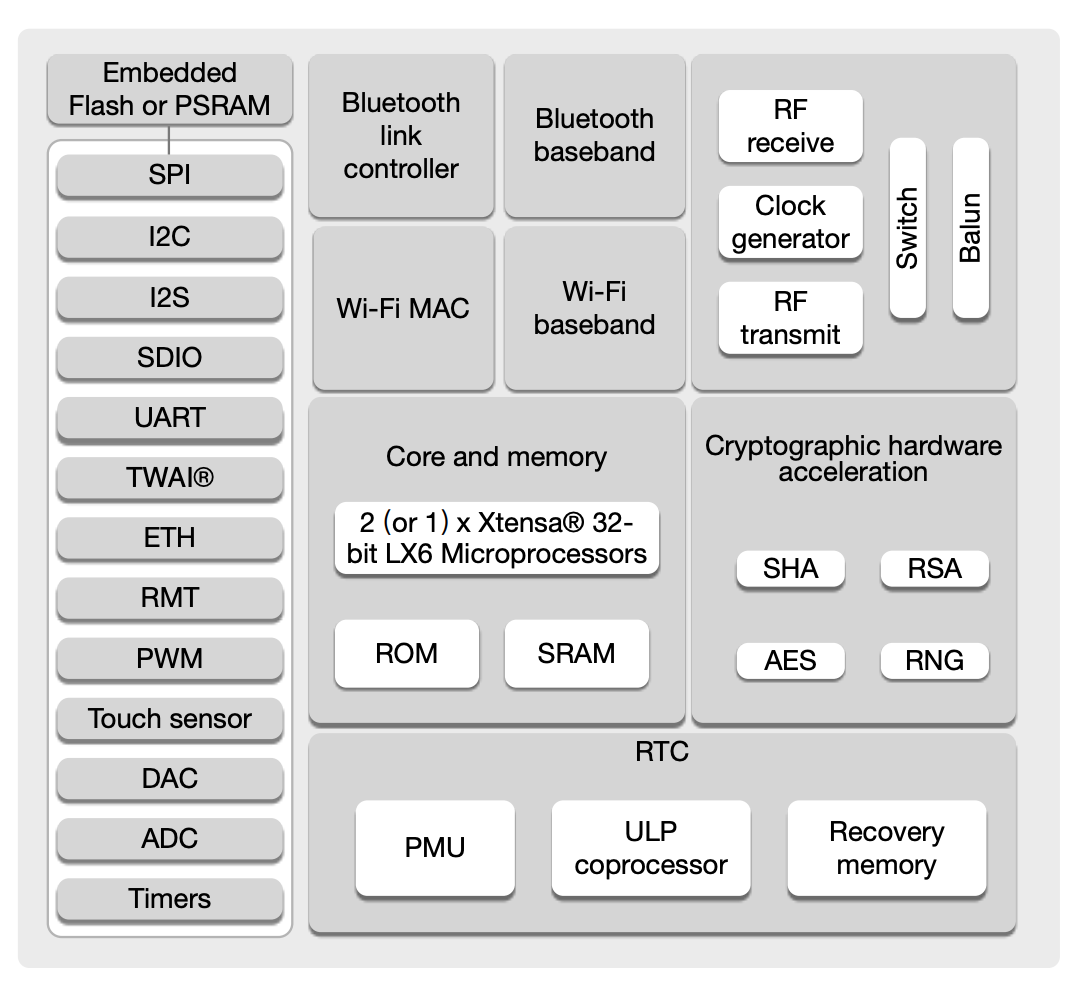
\includegraphics[width=.6\textwidth]{./Figures/esp32hardware.png}
\caption{Diagrama de bloques ESP32.}
\label{fig:diagBloques}
\end{figure}

A su vez, en la familia de ESP32 existen diferentes tipos de módulos [12]. Cada uno presenta pequeñas variaciones de hardware, comandos de integración de firmware y cantidad de pines. En particular, para este trabajo se utiliza el módulo de WROOM. Más específicamente, uno de los tableros de ESP32-devkit [13]. Además, existen diferentes versiones de tableros de desarrollo de WROOM para ESP32-DEVKIT. Por ello, para realizar las conexiones con los sensores, es fundamental tener conocimiento sobre la usabilidad de cada uno de los pines de la placa. En la figura 2.2 [14] es posible observar un diagrama de pines del módulo.\\

\begin{figure}[htpb]
\centering 
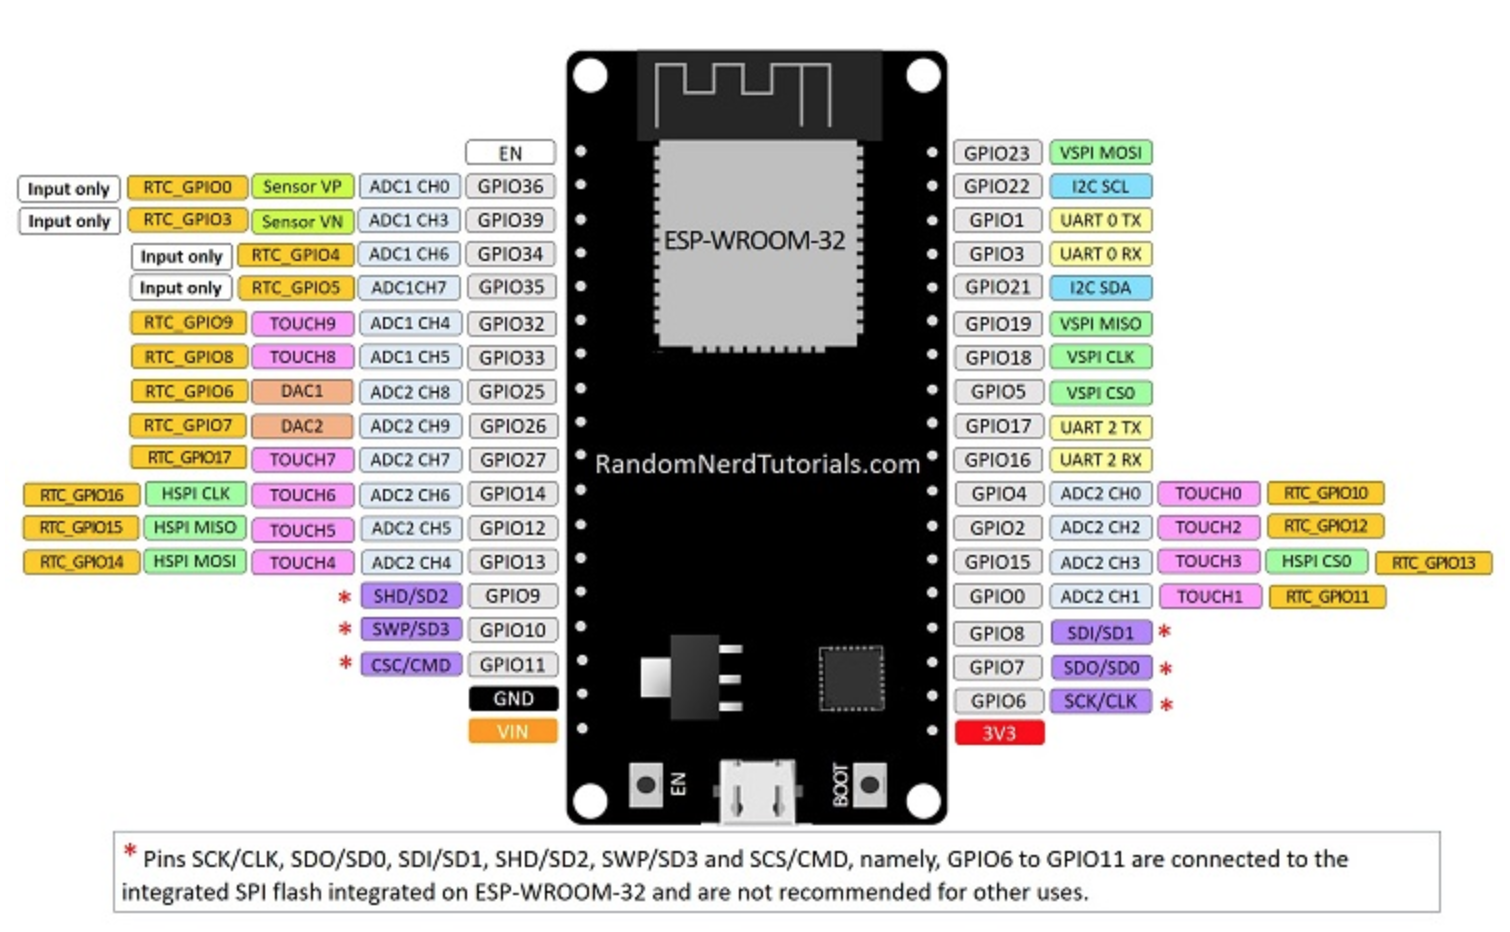
\includegraphics[width=.9\textwidth]{./Figures/esp32pines.png}
\caption{Diagrama pines ESP32.}
\label{fig:diagBloques}
\end{figure}

La selección de este módulo se basó no solo en sus excelentes características de hardware, sino también en las ventajas que ofrece en términos de software. Espressif, el fabricante de la placa, proporciona una amplia variedad de ejemplos de código C en sus repositorios de GitHub [15].\\

\subsection{Sensor de temperatura y humedad relativa DHT22}
Con este sensor se podrá realizar la obtención de valores de temperatura y humedad ambiente. Según se detalla en su hoja de datos [16] ofrece una señal digital confiable y estable.
Este sensor cuenta con 4 pines, de los cuales se utilizarán los siguientes 3 (numeración de izquierda a derecha con el sensor de frente):
\begin{itemize}
\item Pin 1: VDD (alimentación). Deberá recibir de 3,3 a 6 V. Se recomienda colocar un capacitor de 100 nF entre este pin y el pin GND para su protección.
\item Pin 2: DATA. Una vez establecida la conexión, este pin enviará los datos de temperatura y humedad relativa al módulo ESP.
\item Pin 4: GND.\\
\end{itemize}

\subsection{Sensor de humedad en suelo capacitivo analógico V1.2}
Es un sensor que se utiliza para medir la humedad del sustrato. Como se menciona en su hoja de datos [17] es una excelente opción ya que <<está hecho de un material resistente a la corrosión lo que le da una excelente vida útil>>. Este sensor cuenta con un conector de pines con especificaciones muy claras: VCC, GND y AOUT (datos analógicos). Se recomienda utilizar con una potencia de 3,3 a 5 V.

\subsection{ADC ADS1115}
Debido a que el sensor de humedad de suelo tiene mayores pruebas y confiabilidad usando Arduino (incluso en su hoja de datos) se va a agregar un convertidor analógico digital con el ESP32. Se utilizó como fuente de información su hoja de datos [18] y documentación adicional [19]. De esta forma se transformará la señal analógica, del sensor capacitivo, a digital para enviarla a la placa ESP32.

%----------------------------------------------------------------------------------------

\section{Herramientas de software}

Para el desarrollo de software se trabajó con diferentes lenguajes de programación para el backend y el frontend. A su vez, en cada capa se definió el uso de frameworks que provean de funcionalidad base para agilizar el desarrollo. A continuación se detallan  las siguientes tecnologías.

\subsection{Backend con Java y SpringBoot}
Se optó por trabajar con Java [20] como lenguaje de programación, utilizando las bibliotecas y funcionalidades que ofrece el framework de Spring Boot [21]. Con estas tecnologías se realiza:
\begin{itemize}
\item Conexión con la base de datos utilizando MySQL [22].
\item Integración con la capa física.
\item Desarrollo de los endpoints para integración con el frontend.
\item Capa de validación y seguridad (para usuarios y dispositivos).
\end{itemize}

\subsection{Frontend con JavaScript y React}
Con respecto al frontend se definió utilizar JavaScript [23] como lenguaje de programación y el conjunto de bibliotecas de React [24] para el desarrollo de las vistas del sistema. Con estas herramientas se realiza:
\begin{itemize}
\item Bloqueo de URL´s no permitidas sin autenticación.
\item Definición de componentes visuales del sistema para su re utilización.
\item Maquetado con herramientas pre definidas de estilos CSS.
\item Formularios reactivos.
\end{itemize}

%----------------------------------------------------------------------------------------
